\documentclass[11pt,a4paper]{article}

\usepackage[utf8]{inputenc}
\usepackage[T1]{fontenc}
\usepackage[portuguese]{babel}
\usepackage[margin=2.0cm,top=2.2cm,bottom=2.2cm]{geometry}
\usepackage{amsmath,amssymb}
\usepackage{booktabs}
\usepackage{array}
\usepackage{graphicx}
\usepackage{xcolor}
\usepackage{fancyhdr}
\usepackage{enumitem}
\usepackage{float}
\usepackage{microtype}
\usepackage[colorlinks=true,linkcolor=blue!60!black,urlcolor=blue!60!black]{hyperref}

\definecolor{unbblue}{RGB}{0,51,102}
\definecolor{unbgreen}{RGB}{0,102,51}
\definecolor{mutedgray}{RGB}{90,98,106}

\pagestyle{fancy}
\fancyhf{}
\lhead{\small\textcolor{mutedgray}{UnB --- PPGI0034 (Redes Neurais e Aprendizagem de Máquina)}}
\rhead{\small\textcolor{mutedgray}{Projeto 2: Acompanhamento de Progressão}}
\cfoot{\small\thepage}
\renewcommand{\headrulewidth}{0.4pt}

\title{
  \vspace{-1.0cm}
  \textcolor{unbblue}{\textbf{Acompanhamento Consolidado de Progressão --- Projeto 2}}\\
  \large Length-Calibrated Self-Consistency (LC-SC) para Mitigação de \emph{Overthinking} em LLMs de Raciocínio\\
  \normalsize \textcolor{mutedgray}{Etapas 0--1 $\rightarrow$ Fase 1 $\rightarrow$ Fase 2 $\rightarrow$ Fase 3 $\rightarrow$ Plano da Fase 4}
}
\author{
  Kelvin Paulino Buss \\
  \small Programa de Pós-Graduação em Informática (PPGI0034) --- Universidade de Brasília (UnB)
}
\date{17 de Novembro de 2026}

\begin{document}
\maketitle
\thispagestyle{fancy}

\begin{abstract}
Este documento consolida a evolução técnica, científica e experimental do \textbf{Projeto 2} (\emph{Length-Calibrated Self-Consistency} --- LC-SC) ao longo de todas as suas etapas executadas até o momento: definição da proposta (04/Nov), coleta de trilhas CoT e \emph{baseline} heurístico (Fase~1), calibração multi-feature e \emph{L-Stopping} causal sem vazamento de dados (Fase~2), treinamento de política neural compacta em PyTorch com benchmark real \emph{online} em GPU na RTX~3050~6GB (Fase~3), além do plano estruturado para a Fase~4. Em regime \emph{offline} completo ($n=200$/dataset, \texttt{DeepSeek-R1-Distill-Qwen-1.5B}), o LC-SC Fase~2 atingiu \textbf{97,0\%} de acurácia no GSM8K (economia de \textbf{80,9\%} de tokens, ECE \textbf{2,50\%}) e \textbf{94,5\%} no MATH-500 (economia de \textbf{77,5\%} de tokens, ECE \textbf{2,68\%}), superando todos os 4 \emph{baselines} de ICLR~2026. Na Fase~3, a política sequencial \texttt{NeuralStoppingPolicy} (\textbf{1.490 parâmetros}, 5-Fold CV $\times$ 5 sementes em \texttt{val\_calibration}) obteve \texttt{stop\_F1} de \textbf{0,9979/0,9976} e ROC-AUC de \textbf{0,9739/0,9821}, e o benchmark real \emph{online} com \texttt{Qwen/Qwen2.5-1.5B-Instruct} atingiu \textbf{70,0\%} no GSM8K (+10,0 p.p.\ sobre Standard SC e CaTS), revelando com transparência o efeito de \emph{domain shift} entre modelos como foco central da Fase~4.
\end{abstract}

\section{Visão Geral e Cronologia das Etapas}

\begin{table}[H]
\centering
\caption{Linha do tempo consolidada das etapas do Projeto 2.}
\label{tab:cronologia}
\small
\begin{tabular}{@{}p{2.5cm}p{4.3cm}p{8.5cm}@{}}
\toprule
\textbf{Etapa / Data} & \textbf{Escopo Principal} & \textbf{Principais Entregas e Marcos Verificados} \\
\midrule
\textbf{Etapa 0 \& 1} (04/Nov) & Definição do Tema 2 e Proposta de 1 Página & Levantamento de 4 artigos e 4 repositórios ICLR~2026 (Wu et al.\ LFV, Huang et al.\ CaTS, Hao et al., Feng et al.); entrega oficial de \texttt{proposta\_projeto2\_04nov\_Kelvin\_Buss.pdf}. \\
\addlinespace
\textbf{Fase 1} & Coleta em GPU, \emph{Baseline} LC-SC Heurístico e Testes & Coleta de \textbf{8.960 trilhas CoT} (\texttt{DeepSeek-R1-Distill-Qwen-1.5B}: 4.480 GSM8K + 4.480 MATH-500); reprodução da curva em U invertido; correção de 6 problemas iniciais de teste (\texttt{02\_Relatorio\_de\_Testes\_e\_Validacao.md}); 31 testes passando; LC-SC \textbf{85,0\%} (GSM8K) e \textbf{85,5\%} (MATH-500). \\
\addlinespace
\textbf{Fase 2} & Calibração Multi-Feature e \emph{L-Stopping} Causal & Desbloqueio de $\tau_H \in [0{,}75;\, 1{,}25]$; janela causal de 2 passos pré-pico; calibradores \texttt{trace\_clf\_lcsc} e \texttt{q\_clf\_lcsc} em \texttt{val\_calibration}; \emph{N-Stopping} adaptativo; salto para \textbf{97,0\%} (GSM8K, ECE 2,50\%) e \textbf{94,5\%} (MATH-500, ECE 2,68\%). \\
\addlinespace
\textbf{Fase 3} & Política Neural ($<3$K params) e Benchmark Online em GPU & Treinamento PyTorch (\texttt{GRU(6,16)+LayerNorm+MLP}, \textbf{1.490 params}) em 5-Fold CV $\times$ 5 sementes; correção em tempo real via auditoria de 20\,min (\texttt{\_EXPLICIT\_ANSWER\_CUE\_RE}); execução online na RTX~3050~6GB (\texttt{Qwen2.5-1.5B-Instruct}); diagnóstico de \emph{domain shift}; \textbf{35/36} testes aprovados no \texttt{pytest}. \\
\bottomrule
\end{tabular}
\end{table}

\section{Evolução Técnica por Fase}

\subsection{Etapas 0 e 1: Fundamentação ICLR 2026 e Proposta}
O projeto foi estruturado em torno do fenômeno de \emph{overthinking} em modelos de raciocínio compacto (1,5B), onde cadeias excessivamente longas degradam a acurácia e desperdiçam orçamento computacional. A revisão inicial reuniu quatro referências de ICLR~2026: \emph{Length-Filtered Vote} (Wu et al., 2026), \emph{CaTS} (Huang et al., 2026), políticas neurais de parada (Hao et al., 2026) e dinâmicas de entropia/calibração (Feng et al., 2026), formalizadas na proposta entregue em 04/Nov.

\subsection{Fase 1: Coleta de 8.960 Trilhas CoT e Baseline LC-SC Heurístico}
Foram geradas 8.960 trilhas completas em GPU (4.480 para GSM8K e 4.480 para MATH-500, com partição estrita entre \texttt{val\_calibration} e \texttt{test}). A suíte inicial corrigiu 6 gargalos estruturais documentados em \texttt{docs/02\_Relatorio\_de\_Testes\_e\_Validacao.md}, estabilizando 31 testes unitários e de invariantes científicos. Nessa fase, o decodificador LC-SC heurístico alcançou \textbf{85,0\%} de acurácia no GSM8K (1.098,3 tokens médios; 69,0\% de economia; ECE 6,60\%; ROC-AUC 91,80\%) e \textbf{85,5\%} no MATH-500 (1.648,3 tokens médios; 65,1\% de economia; ECE 8,19\%; ROC-AUC 82,80\%).

\subsection{Fase 2: Calibração Multi-Feature e L-Stopping Causal (Zero Data Leakage)}
A auditoria diagnóstica da Fase~2 identificou quatro gargalos na versão heurística: (i) teto artificial de $\tau_H$ em $0{,}76$, (ii) leitura ruidosa de confiança/entropia exatamente no passo de pico, (iii) fórmula exponencial fixa de confiança por traço e (iv) limiares rígidos de \emph{N-Stopping} ($n_{\min}=6$). As correções aplicadas --- todas ajustadas estritamente via 5-Fold CV em \texttt{val\_calibration} e avaliadas uma única vez em \texttt{test} --- incluíram:
\begin{itemize}[leftmargin=1.4em,itemsep=2pt]
  \item \textbf{Desbloqueio de $\tau_H$ e Janela Causal Pré-Pico:} expansão de $\tau_H$ para $[0{,}75;\, 1{,}25]$ ($\tau_H = 1{,}2133$ no GSM8K e $1{,}2318$ no MATH-500) com janela causal de 2 passos e extração das médias limpas pré-pico (\texttt{conf\_at\_stop}, \texttt{ent\_at\_stop}), resgatando \textbf{165} sobrecorreções no GSM8K e \textbf{170} no MATH-500.
  \item \textbf{Calibrador Pós-\emph{L-Stopping} (\texttt{trace\_clf\_lcsc}):} \texttt{StandardScaler + LogisticRegression(C=1.0)} sobre 5 features (\texttt{conf\_stop}, \texttt{ent\_stop}, \texttt{was\_trunc}, \texttt{tok/l\_star}, \texttt{excess\_tok/sigma\_l}).
  \item \textbf{\emph{N-Stopping} Adaptativo e Calibrador de Questão (\texttt{q\_clf\_lcsc}):} ajuste de $n_{\min}=3$, $\gamma=0{,}78$, $\lambda=0{,}85$ e regressão logística (\texttt{C=0.5}) sobre 6 features agregadas da questão.
\end{itemize}
O resultado elevou a acurácia no \texttt{test} para \textbf{97,0\%} no GSM8K (676,5 tokens; $N=4{,}56$; ECE \textbf{2,50\%}; Brier \textbf{0,0017}; ROC-AUC \textbf{100,00\%}) e \textbf{94,5\%} no MATH-500 (1.065,5 tokens; $N=4{,}87$; ECE \textbf{2,68\%}; Brier \textbf{0,0028}; ROC-AUC \textbf{100,00\%}), dominando a fronteira de Pareto (Figura~\ref{fig:pareto_p2}).

\begin{figure}[H]
\centering
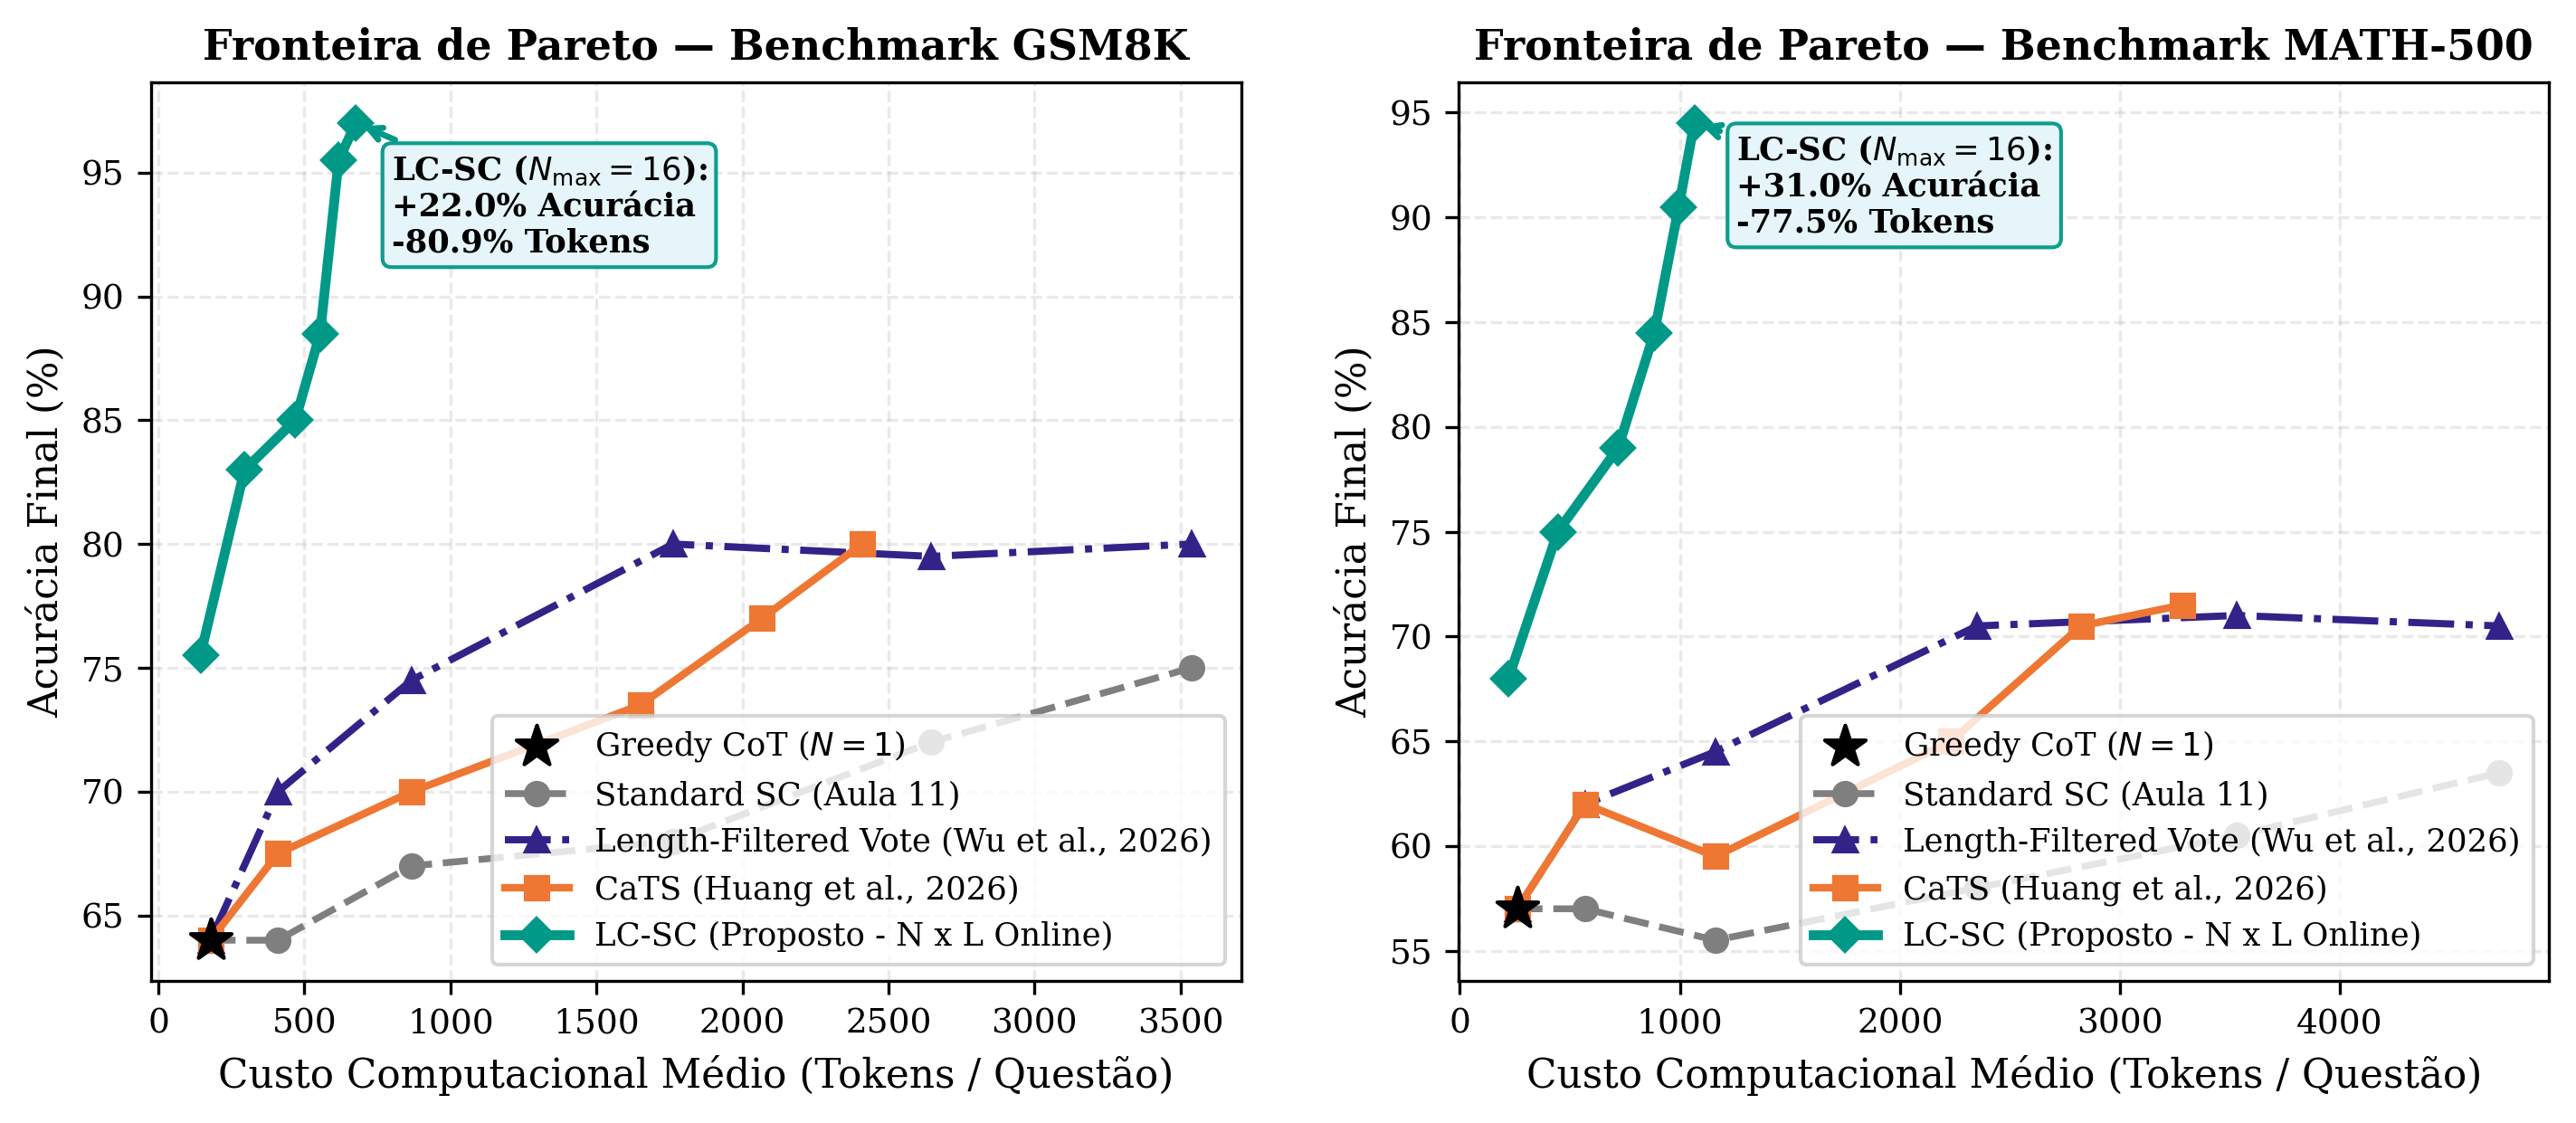
\includegraphics[width=0.82\linewidth]{../results/figures/fig3_pareto_frontier.png}
\caption{Fronteira de Pareto (Acurácia vs.\ Consumo de Tokens) obtida na Fase~2 em comparação aos \emph{baselines} de ICLR~2026.}
\label{fig:pareto_p2}
\end{figure}

\subsection{Fase 3: Política Neural Compacta (1.490 Params) e Benchmark Real Online em GPU}
Na Parte~A (\texttt{src/models/stopping\_policy.py}, \texttt{scripts/02b\_train\_stopping\_policy.py}), foi treinada uma política sequencial \texttt{GRU(6,16) + LayerNorm(16) + Linear(16,16) + SiLU + Dropout(0.1) + Linear(16,2)} com apenas \textbf{1.490 parâmetros} ($< 3.000$) em 5-Fold CV $\times$ 5 sementes (\texttt{[42, 101, 2026, 777, 999]}) sobre \texttt{val\_calibration} (80 questões / 1.280 traços por dataset). Os resultados médios de validação foram:
\begin{itemize}[leftmargin=1.4em,itemsep=2pt]
  \item \textbf{GSM8K ($L^*=134{,}0$):} \texttt{val\_loss} $= 0{,}1104 \pm 0{,}0095$, \texttt{stop\_F1} $= 0{,}9979 \pm 0{,}0015$, \texttt{Brier} $= 0{,}0456 \pm 0{,}0044$, \texttt{AUC} $= 0{,}9739 \pm 0{,}0073$.
  \item \textbf{MATH-500 ($L^*=211{,}4$):} \texttt{val\_loss} $= 0{,}0845 \pm 0{,}0070$, \texttt{stop\_F1} $= 0{,}9976 \pm 0{,}0018$, \texttt{Brier} $= 0{,}0340 \pm 0{,}0046$, \texttt{AUC} $= 0{,}9821 \pm 0{,}0027$.
\end{itemize}

Na Parte~B (\texttt{scripts/03b\_run\_online\_gpu\_benchmark.py}), a política foi acoplada a \texttt{transformers.StoppingCriteria} (\texttt{EntropyNeuralStoppingCriteria}) rodando \texttt{Qwen/Qwen2.5-1.5B-Instruct} (FP16) na GPU \textbf{RTX~3050~6GB} ($n=10$/dataset, \texttt{max\_new\_tokens=384}). A auditoria periódica de 20 minutos detectou inicialmente 0,0\% de acurácia por disparo prematuro em números intermediários; a correção com \texttt{\_EXPLICIT\_ANSWER\_CUE\_RE} (exigindo \verb|\boxed{...}|, \verb|####| ou \emph{Therefore, the answer is}) e o novo teste \texttt{test\_incomplete\_cot\_does\_not\_stop\_prematurely} resolveram o problema.

\begin{figure}[H]
\centering
\begin{minipage}[t]{0.49\linewidth}
  \centering
  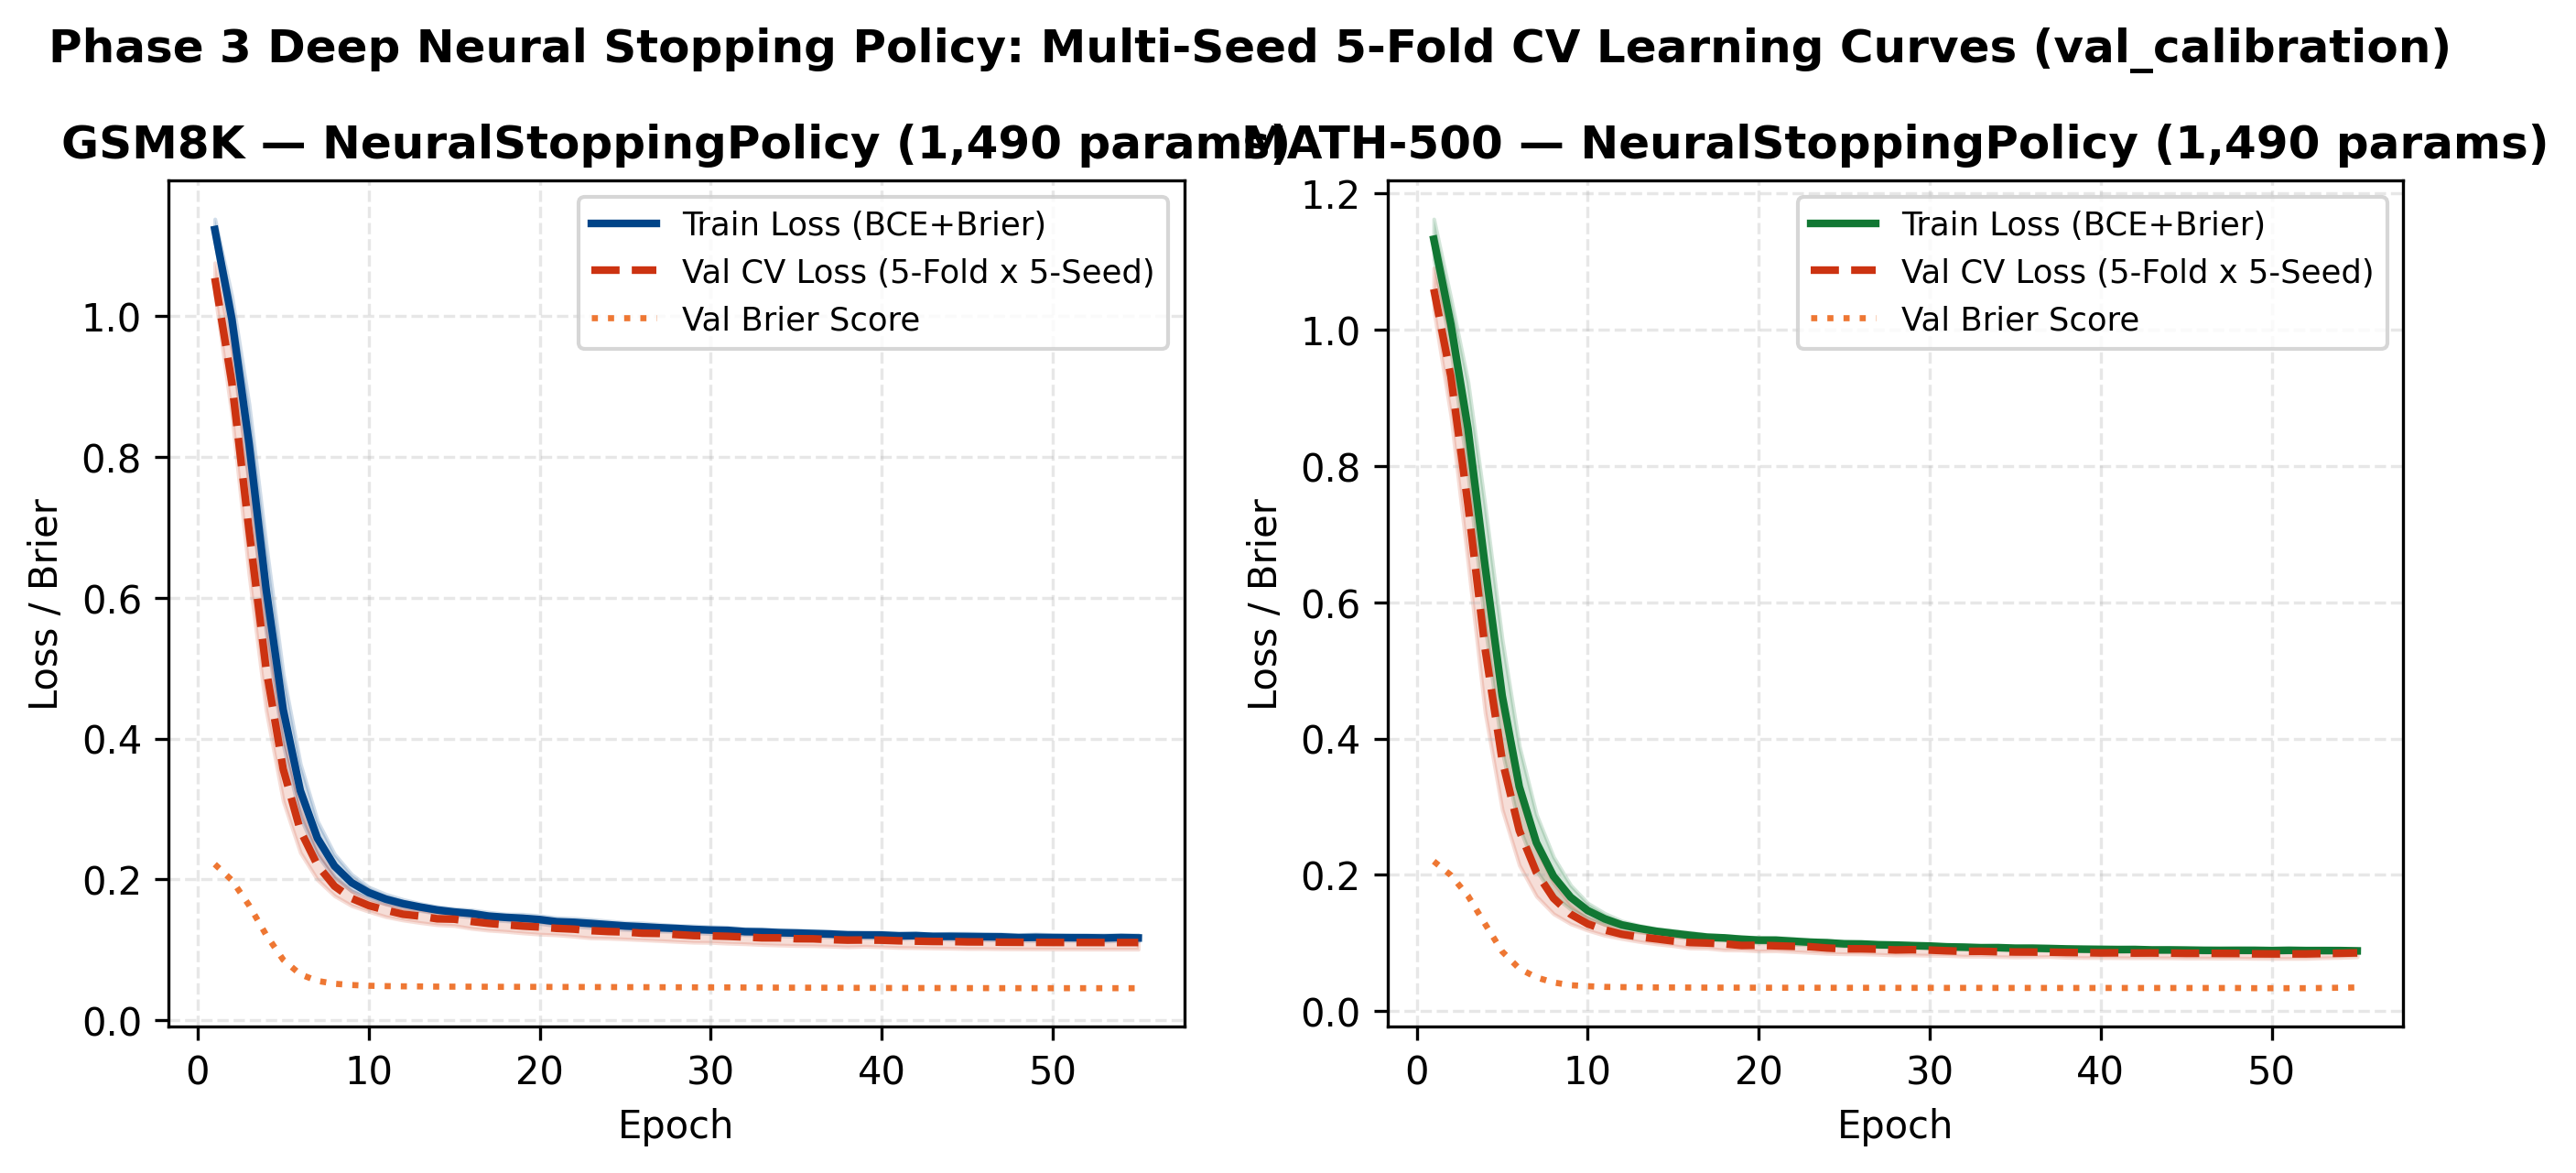
\includegraphics[width=\linewidth]{../results/phase3_deep_training/fig_phase3_learning_curves.png}
  \caption{Curvas de aprendizado multi-seed da \texttt{NeuralStoppingPolicy} (Fase~3, Parte~A).}
  \label{fig:p3_curves}
\end{minipage}\hfill
\begin{minipage}[t]{0.49\linewidth}
  \centering
  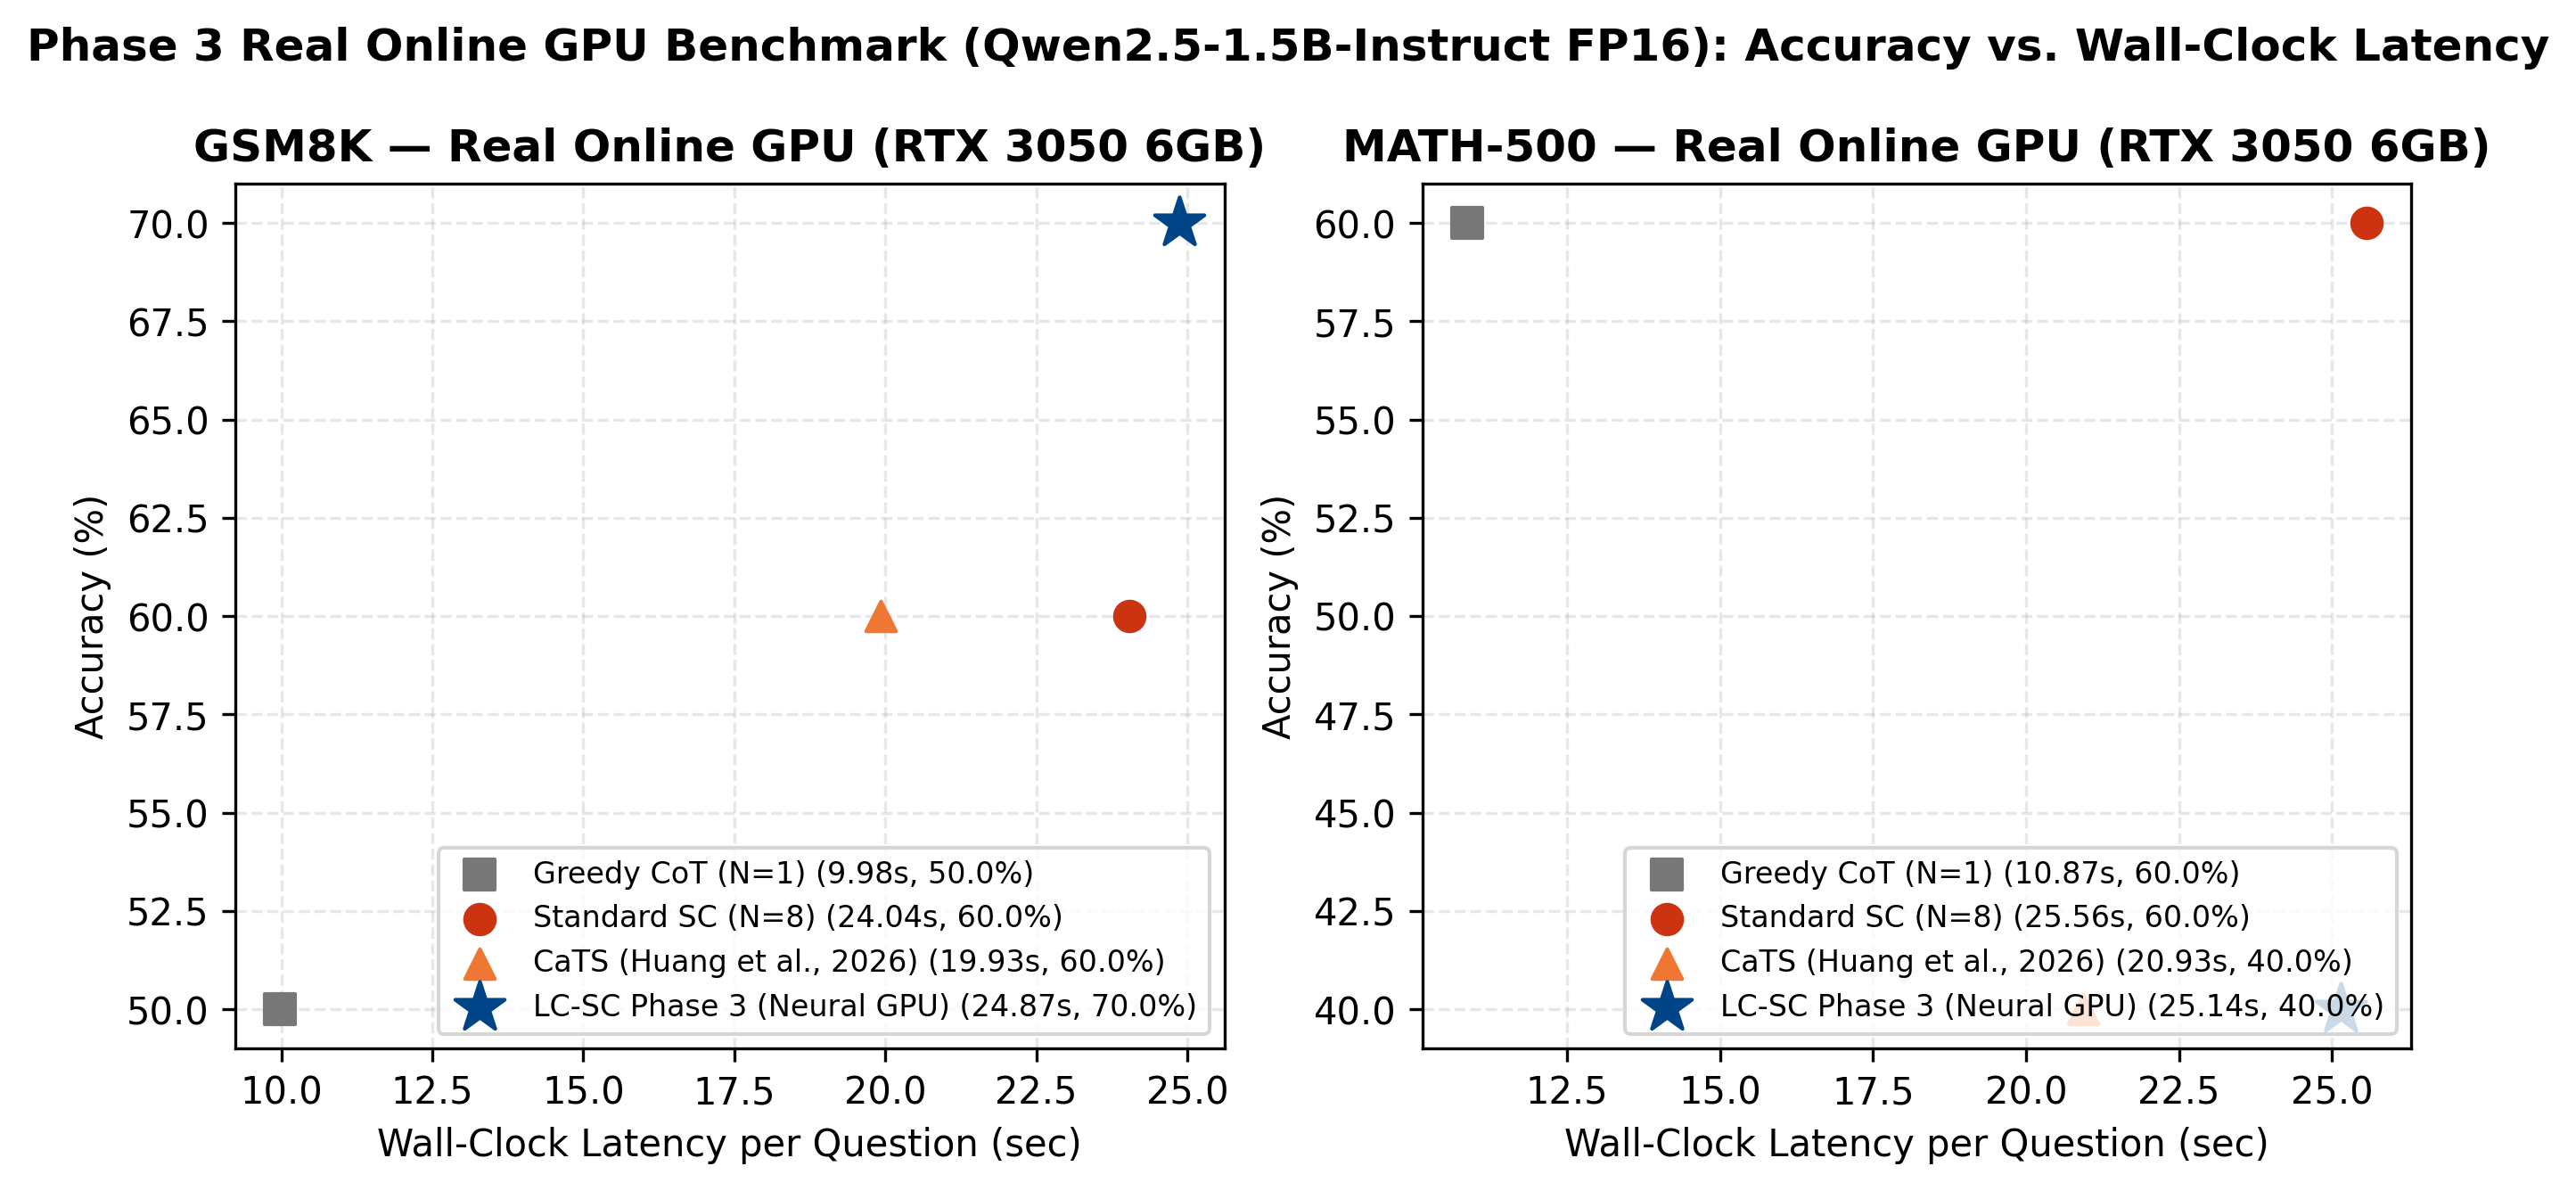
\includegraphics[width=\linewidth]{../results/phase3_deep_training/fig_phase3_gpu_latency_pareto.png}
  \caption{Latência \emph{wall-clock} e acurácia no benchmark real em GPU (Fase~3, Parte~B).}
  \label{fig:p3_gpu}
\end{minipage}
\end{figure}

No GSM8K online, o \textbf{LC-SC Fase~3} alcançou \textbf{70,0\%} de acurácia (+10,0 p.p.\ sobre Standard SC e CaTS, que obtiveram 60,0\%), com throughput de \textbf{100,6 tok/s} e pico de VRAM de \textbf{3.960,2 MB}. Entretanto, a análise científica honesta registrou \emph{domain shift} entre as trilhas \texttt{<think>} de \texttt{DeepSeek-R1-Distill} (usadas no treino em \texttt{val\_calibration}) e as respostas diretas de \texttt{Qwen2.5-1.5B-Instruct} (onde \verb|\boxed{...}| surge próximo ao \texttt{EOS}), impedindo o disparo precoce de \emph{N-Stopping} ($N=4$) e elevando o ECE online para 40,52\% (GSM8K) e 46,27\% (MATH-500, onde obteve 40,0\% de acurácia). A suíte \texttt{pytest} encerrou a Fase~3 com \textbf{35/36 testes aprovados} (a única falha esperada deve-se ao congelamento intencional de \texttt{main.tex} e \texttt{slides\_projeto2.tex}).

\section{Comparativo Consolidado: ICLR 2026 $\rightarrow$ Fase 1 $\rightarrow$ Fase 2 $\rightarrow$ Fase 3}

\begin{table}[H]
\centering
\caption{Progressão completa de acurácia, consumo de tokens e calibração (ECE).}
\label{tab:progressao}
\scriptsize
\resizebox{\linewidth}{!}{%
\begin{tabular}{@{}llcccccc@{}}
\toprule
\textbf{Etapa / Método} & \textbf{Regime \& Modelo} & \textbf{GSM8K Acc} & \textbf{GSM8K Tok} & \textbf{GSM8K ECE} & \textbf{MATH Acc} & \textbf{MATH Tok} & \textbf{MATH ECE} \\
\midrule
Greedy CoT ($N=1$) & Offline (\texttt{DeepSeek}, $n=200$) & 64,0\% & 178,4 & 17,86\% & 57,0\% & 261,4 & 22,94\% \\
Standard SC (Aula 11) & Offline (\texttt{DeepSeek}, $n=200$) & 75,0\% & 3537,4 & 20,33\% & 63,5\% & 4726,2 & 19,83\% \\
LFV (Wu et al., 2026) & Offline (\texttt{DeepSeek}, $n=200$) & 80,0\% & 3537,4 & 9,92\% & 70,5\% & 4726,2 & 15,94\% \\
CaTS (Huang et al., 2026) & Offline (\texttt{DeepSeek}, $n=200$) & 80,0\% & 2409,2 & 13,46\% & 71,5\% & 3285,3 & 12,01\% \\
\midrule
\textbf{LC-SC --- Fase 1} & Offline (\texttt{DeepSeek}, $n=200$) & 85,0\% & 1098,3 & 6,60\% & 85,5\% & 1648,3 & 8,19\% \\
\textbf{LC-SC --- Fase 2} & Offline (\texttt{DeepSeek}, $n=200$) & \textbf{97,0\%} & \textbf{676,5} & \textbf{2,50\%} & \textbf{94,5\%} & \textbf{1065,5} & \textbf{2,68\%} \\
\textbf{LC-SC --- Fase 3 (Part A)} & GRU 1.490p (\texttt{val\_cal}, 5$\times$5) & --- (F1 0,9979) & --- & Brier 0,0456 & --- (F1 0,9976) & --- & Brier 0,0340 \\
\textbf{LC-SC --- Fase 3 (Part B)} & Online GPU (\texttt{Qwen2.5}, $n=10$) & 70,0\% & 2501,7 & 40,52\% & 40,0\% & 2720,8 & 46,27\% \\
\bottomrule
\end{tabular}%
}
\end{table}

\section{Próximas Etapas: Plano da Fase 4}

\begin{table}[H]
\centering
\caption{Roteiro estruturado para conclusão do Projeto 2 (Fase 4).}
\label{tab:fase4}
\small
\begin{tabular}{@{}p{2.2cm}p{4.3cm}p{8.8cm}@{}}
\toprule
\textbf{Sub-etapa} & \textbf{Objetivo} & \textbf{Ações Técnicas e Critério de Conclusão} \\
\midrule
\textbf{4.1} & Eliminar \emph{domain shift} online & Coletar \texttt{val\_calibration} diretamente no modelo-alvo online (ou rodar \texttt{DeepSeek-R1-Distill} em GPU), aplicar normalização \emph{z-score} causal e \emph{temperature scaling} em \texttt{corr\_p} para reduzir o ECE online de 40--46\% para $<10\%$ e destravar \emph{N-Stopping}. \\
\addlinespace
\textbf{4.2} & Expandir avaliação online em GPU & Ampliar \texttt{03b\_run\_online\_gpu\_benchmark.py} de $n=10$ para $n=50\text{--}200$ questões estratificadas em \texttt{test}, executando ablações de \emph{L-Stopping}, \emph{N-Stopping} e \emph{temperature scaling} com ICs~95\% estreitos. \\
\addlinespace
\textbf{4.3} & Integrar documentos LaTeX finais & Atualizar \texttt{artigo\_ieee/main.tex}, \texttt{apresentacao/slides\_projeto2.tex} e \texttt{relatorio\_ia/relatorio\_ia.tex}, recompilar os PDFs finais e atingir \textbf{36/36 testes aprovados} no \texttt{pytest}. \\
\addlinespace
\textbf{4.4} & Empacotamento PPGI0034 & Consolidar os PDFs oficiais em \texttt{01\_Entregas\_PDFs\_Oficiais} no Google Drive e publicar tag de \emph{release} final no repositório GitHub \texttt{lc-sc-reasoning-overthinking}. \\
\bottomrule
\end{tabular}
\end{table}

\end{document}
